\chapter{Použitý model}

\begin{figure}
	\caption{Části adresy URL}\label{url_parts}
	\centering
	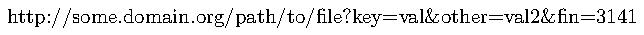
\includegraphics{images/url/url.pdf}
\end{figure}

\begin{figure}
	\caption{Model adresy URL}\label{url_model}
	\centering
	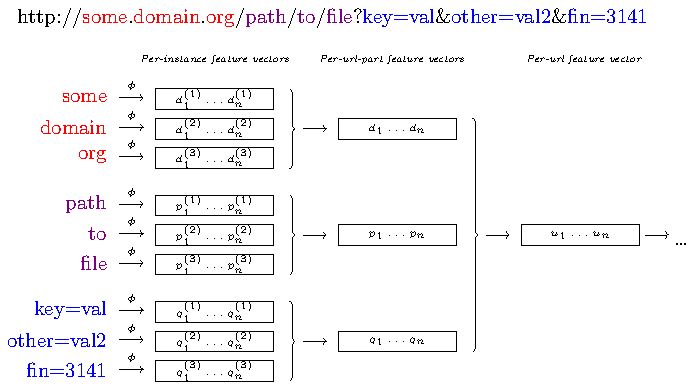
\includegraphics{images/model/model.pdf}
\end{figure}

\section{Řešená úloha}
Řešená úloha, jejímž cílem je klasifikace síťových spojení, vyhovuje formalismu, popsaném v \ref{used_formalism}. Cílem je navrhnout klasifikační funkci, která pro danou vstupní URL adresu (\textit{\textenglish{uniform resource locator}}, srov. \cite{berners-lee_uniform_1994}) rozhodne, zda spojení mířící na takovouto adresu pochází z běžné aktivity uživatele-klienta, či zda se jedná o spojení, které vytvořil nějaký nežádoucí software. Pro tento účel je nejprve adresa URL rozdělena na tři části, a to sice doménu, (\textit{\textenglish{domain}}), cestu (\textit{\textenglish{path}}) a dotaz (\textit{\textenglish{query}}). Na obrázku \ref{url_parts} lze vidět toto rozdělení na příkladu, červeně je vyznačena doména, fialově cesta a modře dotaz. Dále je pak každá část adresy rozdělena na několik podčástí. Doména je rozdělena podle znaku "." (tečka), tedy podle jednotlivých úrovní domén. Cesta je rozdělena podle znaku "/" (lomítko), tedy na jednotlivé adresáře a soubory. Dotaz je rozdělen podle znaku "\&" (ampersand), tedy na páry klíč-hodnota. Na všechny takto vytvořené řeťezce je aplikována \todo{Jaká? - Odkaz na další kapitolu}nějaká funkce \( \psi : U^* \to \BPfield R^n \), kde \( U \) je abeceda všech znaků \todo{Odkaz na standard?}Unicode. Tím je definován prostor vstupních objektů jako
\begin{equation}
	\BPspace X_1 = \psi \left( U^* \right) \subset \BPfield R^n
\end{equation}
V prostoru \( \BPspace X \) jsou tedy vektory příznaků všech částí adresy. Prostor \( \BPspace B_1 \) je konstruován tak, že každá taška v \( \BPspace B_1 \) odpovídá příznakům jedné části (domény, cesty nebo dotazu) jedné adresy. Potom podle formalismu nastíněného v \ref{used_formalism} lze najít vkládající funkci \( \phi_1 : \BPspace B_1 \to \BPspace X_2 \). Dále je pak konstruován prostor \( \BPspace B_2 \) tak, že každá taška v \( \BPspace B_2 \) odpovídá příznakům jedné adresy, tedy platí
\begin{equation}
	\left( \forall b \in \BPspace B_2 \right) \left( \left| b \right| \leq 3 \right)
\end{equation}
Znovupoužitím formalismu z \ref{used_formalism} lze definovat vkládající funkci \( \phi_2 : \BPspace B_2 \to \BPspace X_3 \). Celý tento postup je graficky znázorněn na obrázku \ref{url_model}

\todo{Expandovat? Vynechat?}Alternativně by bylo možné definovat prostor \( \hat{\BPspace B} \) tak, že každá taška by odpovídala přímo všem příznakům jedné adresy URL. Tento přístup by produkoval jednodušsí jednovrstevý formalismus a tedy jednodušsí modely, avšak nezachycoval by inherentní rozdíl ve funkci jednotlivých částí adresy. Proto byl zvolen tento dvojvrstvý, hierarchický model.

\section{Model}
Při použití značení z \eqref{net_pooling} nechť
\begin{equation}
	\phi_1 : \BPspace B_1 \to \BPspace X_2 : b \mapsto g_1 \left( \left\{ k_1 \left( x \right) \middle| x \in b \right\} \right)
\end{equation}
kde \( g_1 : \bigcup_{k = 1}^{\infty} \left( \BPfield R^n \right)^k \to \BPfield R^n \) je předem definovaná funkce a \( k_1 : \BPfield R^n \to \BPfield R^n \) je funkce definovaná neuronovou síťí. Protože dobře definovaná adresa URL nemusí obsahovat všechny tři části (doména, cesta, dotaz), pokud některá z částí není přítomna, je považována za prázdný řeťězec. Díky tomu platí
\begin{equation}
	\left( \forall b \in \BPspace B_2 \right) \left( \left| b \right| = 3 \right)
\end{equation}
Díky tomuto rozšíření lze definovat funkci \( \phi_2 : \left( \BPfield R^n \right)^3 \to \BPfield R^{3n} \) jako
\begin{equation}
	\phi_2 : \left( x_1^{(1)}, \dots, x_n^{(1)} \right), \left( x_1^{(2)}, \dots, x_n^{(2)} \right), \left( x_1^{(3)}, \dots, x_n^{(3)} \right) \mapsto \left( x_1^{(1)}, \dots, x_n^{(1)}, x_1^{(2)}, \dots, x_n^{(2)}, x_1^{(3)}, \dots, x_n^{(3)} \right)
\end{equation}
Tedy \( \phi_2 \) je pouze konkatenací.

Protože dobře definovaná adresa url nemusí obsahovat všechny tři části (doména, cesta, dotaz), pokud některá z částí není přítomna, je považována za prázdný řeťězec. Díky tomu platí
\begin{equation}
	\left( \forall b \in \BPspace B_2 \right) \left( \left| b \right| = 3 \right)
\end{equation}
Klasifikační funkce \( f : \BPspace X_3 \to \BPspace Y \) je definovaná neuronovou síťí, která je trénovaná společně se sítí definující funkci \( k_1 \).
\todo{Kam tohle?}\begin{align}
	\BPspace X_1 &= \BPfield R^n \\
	\BPspace X_2 &= \BPfield R^n \\
	\BPspace X_3 &= \BPfield R^{3n}
\end{align}

\section{Trénovací a testovací data}

